\documentclass[xcolor=dvipsnames,10pt]{beamer}

\usetheme[presnum=05]{u18fest}

\subtitle{Marco Bayesiano para el análisis de datos,\\
  calibración de parámetros y modelamiento inverso}
\title{Modelamiento probabilístico}%
\institute{Universidad Industrial de Santander}%
\date{U18 Fest}

\usepackage{pgfplots}
\usetikzlibrary{positioning}

\begin{document}

\begin{frame}[noframenumbering]
  \titlepage
\end{frame}

\begin{frame}
  \frametitle{Teorema de Bayes}
  \begin{itemize}
  \item \textbf{Objetivo}: Modelar datos
  \item Si tenemos observaciones $y$ de un observable $Y$ y un modelo de las observaciones parametrizado por $\Theta$, podemos calcular la distribución de los parámetros dadas las observaciones usando
  \end{itemize}
  \begin{equation*}
    p(\theta \mid y) = \frac{p(y \mid \theta) p(\theta)}{p(y)} = \frac{p(y \mid \theta) p(\theta)}{\int p(y \mid \theta) p(\theta) \, \symrm{d} \theta}
  \end{equation*}
\end{frame}
%
\begin{frame}
  \frametitle{Nomenclatura}
  \begin{equation*}
    p(\theta \mid y) = \frac{p(y \mid \theta) p(\theta)}{p(y)} = \frac{p(y \mid \theta) p(\theta)}{\int p(y \mid \theta) p(\theta) \, \symrm{d} \theta}
  \end{equation*}
  \vskip1em
  \begin{overprint}
    \onslide<1>
    \begin{itemize}
      \setlength{\itemsep}{5mm}
    \item $p(y \mid \theta)$: \textbf{Verosimilitud}\\
      El valor de la pdf de las observaciones dado el valor específico $\Theta = \theta$ de los parámetros.
      La verosimilitud indica qué tan posible es observar las (uh) observaciones dado $\theta$
    \item $p(\theta)$: \textbf{(Distribución) Anterior}\\
      Codifica la información disponible o suposiciones acerca de la distribución de probabibilidad de $\Theta$, i.e, indica qué valores de $\Theta$ son más o menos probables de acuerdo a la información \emph{a priori}
    \end{itemize}
    \onslide<2>
    \begin{itemize}
      \setlength{\itemsep}{5mm}
    \item $p(\theta \mid y)$: \textbf{(Distribución) Posterior}\\
      pdf de $\Theta$ dadas las observaciones, i.e., indica qué valores de $\Theta$ son más o menos probables de acuerdo a las observaciones y la información \emph{a priori}
    \item $p(y) = \int p(y \mid \theta) p(\theta) \, \symrm{d} \theta$: \textbf{Verosimilitud marginal}\\
      Indica qué valores del observable $Y$ son más o menos posibles dada la información \emph{a priori} acerca de los parámetros del modelo
    \end{itemize}
  \end{overprint}
\end{frame}
%
\begin{frame}
  \frametitle{Nomenclatura}
  \begin{itemize}
  \item Para calcular la distribución posterior sólo hace especificar las verosimilitud $p(y \mid \theta)$ y la distribución anterior, i.e, la distribución conjunta
    \begin{equation*}
      p(y, \theta) = p(y \mid \theta) p(\theta)
    \end{equation*}
  \item Ésta distribución conjunta se conoce como el \emph{modelo probabilístico}
  \end{itemize}
\end{frame}
%
\begin{frame}
  \frametitle{Tareas de regresión}
  \begin{itemize}
  \item Queremos analizar la dependencia de un observable $Y$ en una variable explanatoria $x$ utilizando un modelo parametrizado por $\Theta$
  \item Dadas las observaciones $(X, y)$, podemos calcular la distribución de los parámetros:
  \end{itemize}
  \begin{equation*}
    p(\theta \mid y, X) = \frac{p(y \mid X, \theta) p(\theta)}{p(y \mid X)} = \frac{p(y \mid X, \theta) p(\theta)}{\int p(y \mid X, \theta) p(\theta) \, \symrm{d} \theta}
  \end{equation*}
  donde
  \begin{itemize}
  \item $p(y \mid X, \theta)$: Verosimilitud
  \item $p(\theta)$: Anterior
  \item $p(\theta \mid y, X)$: Posterior
  \end{itemize}
\end{frame}
%
\begin{frame}
  \pythonframe
\end{frame}
%
\begin{frame}
  \frametitle{Regresión lineal ordinaria}
  \begin{itemize}
  \item Tenemos un observable $Y$, que se asume contínuo y $k$ variables explanatorias $x = (x_1, x_2, \dots, x_3)$
  \item Un número $n$ de observaciones de la forma
    \begin{equation*}
      y =
      \begin{bmatrix}
        y_1\\y_2\\\vdots\\y_i\\\vdots\\y_n
      \end{bmatrix}, \quad%
      X = \begin{bmatrix}
        x_{11} & x_{12} & \hdots & x_{1k}\\
        x_{21} & x_{22} & \hdots & x_{2k}\\
        \vdots & & & \vdots\\
        x_{i1} & x_{i2} & \hdots & x_{ik}\\
        \vdots & & & \vdots\\
        x_{n1} & x_{n2} & \hdots & x_{nk}\\
      \end{bmatrix}
    \end{equation*}
  \item Modelo lineal para la esperanza de las observaciones
    \begin{align*}
      \mathbb{E}(y_i \mid X, \beta) &= \alpha + x_{i1} \beta_1 + x_{i2} \beta_2 + \dots \beta_k x_{ik}\\
      \mathbb{E}(y \mid X, \beta) &= \alpha + X \beta
    \end{align*}
  \end{itemize}
\end{frame}
%
\begin{frame}
  \frametitle{Verosimilitud normal}
  \begin{itemize}
  \item Para modelar las observaciones, asumimos que cada observación es independiente, y modelada como una variable aleatoria normal con la esperanza dada por el modelo lineal y una cierta varianza
    \begin{equation*}
      p(y_i \mid X, \beta) = \mathcal{N}(y \mid \alpha + X_{i \cdot} \beta, \sigma)
    \end{equation*}
    \begin{figure}
      \centering
      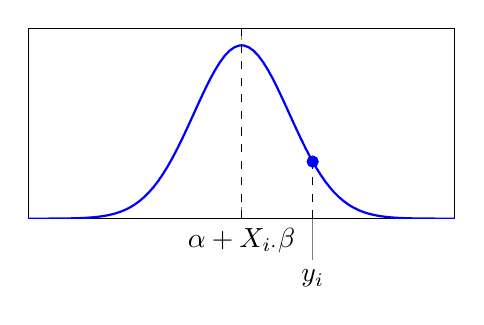
\begin{tikzpicture}
        \begin{axis}[ymin=0, xmin=-3, xmax=3, height=4cm, width=7cm, %
          extra tick style={%
            tick align=outside, tick pos=left, grid style={dotted,black}%
          }, %
          extra x tick style={%
            major tick length=1.25\baselineskip%
          }, %
          extra y tick style={%
            major tick length=2.5em%
          }, %
          extra x ticks={1.0}, extra x tick labels={$y_i$}, xtick={0.0}, xticklabel={$\alpha + X_{i \cdot} \beta$}, ytick={\empty} ]
          \addplot [samples=150, no markers, blue, thick] {exp{-0.5*x^2}/sqrt{2*pi}};%
          \addplot[mark=*,color=blue] coordinates {(1.0, exp{-0.5}/sqrt{2*pi})};%
          \draw [dashed] (axis cs: 1.0, 0.0) -- (axis cs: 1.0, exp{-0.5}/sqrt{2*pi});%
          \draw [dashed] (axis cs: 0.0, 0.0) -- (axis cs: 0.0, 1 / sqrt{2 * pi});%
        \end{axis}
      \end{tikzpicture}
    \end{figure}
  \item La distribución conjunta de las observaciones es
    \begin{equation*}
      p(y \mid X, \beta) = \prod^n_{i = 1} p(y_i \mid X, \beta) = \mathcal{N}(y \mid \alpha + X \beta, \sigma^2 I)
    \end{equation*}
  \end{itemize}
\end{frame}

\end{document}

% Local Variables:
% TeX-master: t
% TeX-engine: luatex
% ispell-local-dictionary: "spanish"
% End:
